% Made up for the tikra gallery: two vectors and their sum, by the parallelogram. In the
% playground, drag the tip of u or of v; the tip of u + v moves both.
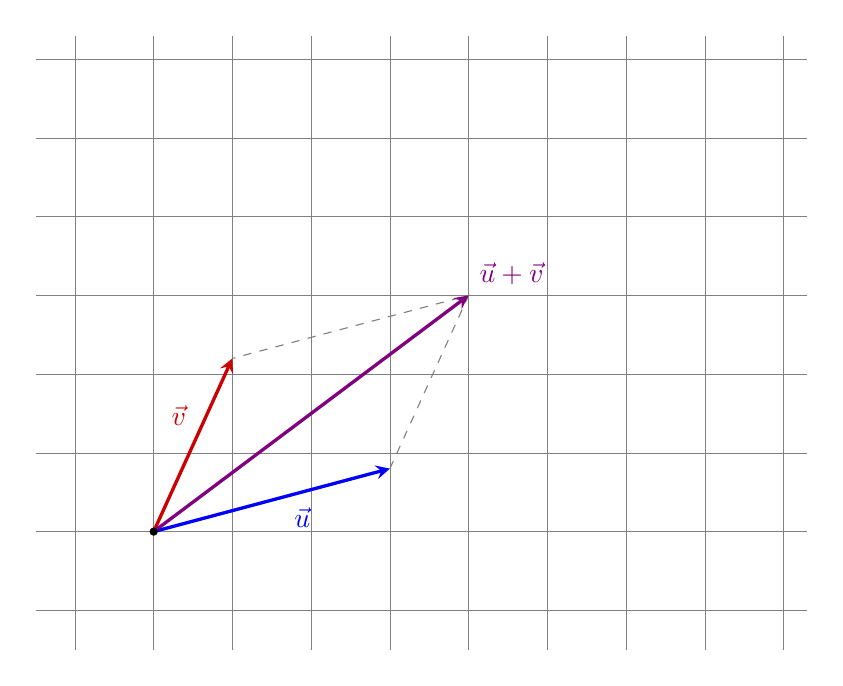
\begin{tikzpicture}[>=stealth]
  \def\ux{3}   % u, x, -1..4
  \def\uy{0.8} % u, y, -1..3
  \def\vx{1}   % v, x, -1..4
  \def\vy{2.2} % v, y, -1..3
  \useasboundingbox (-1.6,-1.6) rectangle (8.4,6.4);
  \draw[help lines, step=1] (-1.5,-1.5) grid (8.3,6.3);
  \coordinate (O) at (0,0);
  \coordinate (u) at (\ux,\uy);
  \coordinate (v) at (\vx,\vy);
  \coordinate (u+v) at ({\ux+\vx},{\uy+\vy});
  \draw[dashed, gray] (u) -- (u+v) -- (v);
  \draw[->, very thick, blue] (O) -- (u) node[pos=0.55, below right] {$\vec u$};
  \draw[->, very thick, red!80!black] (O) -- (v) node[pos=0.55, above left] {$\vec v$};
  \draw[->, very thick, violet] (O) -- (u+v) node[above right] {$\vec u + \vec v$};
  \fill (O) circle (1.5pt);
\end{tikzpicture}
